\documentclass[11pt]{article}
\usepackage{amsmath,textcomp,amssymb,geometry,graphicx,enumerate}
\usepackage{tikz}
\usepackage{pgfplots}
\pgfplotsset{compat=1.18}


\def\Name{Kartikeya Sharma}  % Your name
\def\SID{3037376860}  % Your student ID number
\def\Homework{8 } % Number of Homework
\def\Session{Fall 2024}


\title{COMPSCI 170 Fall 2024 --- Homework \Homework Solutions}
\author{\Name, SID \SID}
\markboth{CS70--\Session\  Homework \Homework\ \Name}{CS170 -- \Session\ Homework \Homework\ \Name}
\pagestyle{myheadings}
\date{\today}

\newenvironment{qparts}{\begin{enumerate}[{(}a{)}]}{\end{enumerate}}
\def\endproofmark{$\Box$}
\newenvironment{proof}{\par{\bf Proof}:}{\endproofmark\smallskip}

\textheight=9in
\textwidth=6.5in
\topmargin=-.75in
\oddsidemargin=0.25in
\evensidemargin=0.25in


\begin{document}

\maketitle

\section*{Q1 Study Group}

\textbf{none}



\newpage


\section*{Q2 Knightmare}

We are tasked with finding the number of ways to place knights on an \( X \times Y \) chessboard such that no two knights attack each other. Knights move in an L-shaped pattern (2x1) in any direction. The goal is to compute the number of valid knight placements modulo 1789, with the time complexity \( O(2^{3Y} \cdot XY) \).

\subsection*{Part 1: Function Definition}

Define the function \( f(r, \text{mask}) \), where:
\begin{itemize}
    \item \( r \) is the current row (from 0 to \( X-1 \)).
    \item \( \text{mask} \) is a bitmask of size \( Y \) representing the knight placements in row \( r \). Each bit in \( \text{mask} \) corresponds to a column, with a 1 indicating a knight is placed in that column and 0 indicating it is empty.
\end{itemize}

The function \( f(r, \text{mask}) \) gives the number of ways to place knights from row 0 to row \( r \), with the configuration of knights in row \( r \) represented by \( \text{mask} \), and no knights attacking each other. We seek to find the sum of valid knight placements for row \( X-1 \), i.e.,
\[
\sum_{\text{mask}} f(X-1, \text{mask}),
\]
where each \( \text{mask} \) represents a valid knight configuration in the last row.

\subsection*{Part 2: Recurrence Relation}

The recurrence relation for \( f(r, \text{mask}) \) is:
\[
f(r, \text{mask}) = \sum_{\text{prev\_mask}} f(r-1, \text{prev\_mask}) \quad \text{if} \ \text{mask} \ \text{and} \ \text{prev\_mask} \ \text{are valid transitions}.
\]

Where:
\begin{itemize}
    \item \( \text{prev\_mask} \) is a valid configuration for row \( r-1 \).
    \item The transition between \( \text{mask} \) and \( \text{prev\_mask} \) is valid if no knights in row \( r \) (as represented by \( \text{mask} \)) can attack knights in row \( r-1 \) (as represented by \( \text{prev\_mask} \)).
\end{itemize}

\textbf{Base Case:}
\[
f(0, \text{mask}) = 1 \quad \text{for all valid knight configurations in row 0}.
\]

This initializes the number of ways to place knights in the first row, assuming that each \( \text{mask} \) represents a valid configuration.

\subsection*{Part 3: Proof of Correctness}

We use induction to prove that the recurrence correctly solves the problem.

\textbf{Base Case:} For \( r = 0 \), the function is initialized with \( f(0, \text{mask}) = 1 \) for all valid configurations, which correctly counts the number of ways to place knights in row 0.

\textbf{Inductive Hypothesis:} Assume that for row \( r-1 \), the function \( f(r-1, \text{mask}) \) correctly counts the number of valid knight placements up to row \( r-1 \).

\textbf{Inductive Step:} For row \( r \), the number of valid configurations is computed by summing over all valid configurations in row \( r-1 \) that can transition to the current row \( r \). The validity check ensures that no knights in row \( r-1 \) can attack knights in row \( r \). Thus, the recurrence relation counts all valid knight placements up to row \( r \), ensuring correctness.

By induction, \( f(r, \text{mask}) \) correctly computes the number of ways to place knights up to row \( r \).

\subsection*{Part 4: Time and Space Complexity}

\textbf{Time Complexity:} The number of possible knight configurations for a row of size \( Y \) is \( 2^Y \), since each column can either contain a knight (1) or not (0). For each row, we check all valid transitions between configurations of the current and previous row, which requires \( 2^Y \times 2^Y = 2^{2Y} \) transitions per row. As there are \( X \) rows, the total time complexity is:
\[
O(2^{2Y} \cdot X) = O(2^{3Y} \cdot XY).
\]

\textbf{Space Complexity:} The dynamic programming table \( f(r, \text{mask}) \) has \( X \) rows and \( 2^Y \) possible configurations per row. Thus, the space complexity is:
\[
O(X \cdot 2^Y).
\]

If we only store the current and previous rows in a bottom-up manner, the space complexity can be reduced to \( O(2^Y) \).

\textbf{Modulo Operation:} All calculations are taken modulo 1789, as required by the problem, to prevent overflow and ensure the result is correct within the given modulus.


\newpage


\section*{Q3 Max Independent Set Again}

Given a tree \( T \) with \( n \) nodes, a root \( r \), and weights \( W[v] \) associated with each vertex \( v \). The task is to find the maximum possible weight of any \( k \)-independent set in \( T \). A \( k \)-independent set is a subset \( S \) of \( T \) with exactly \( k \) nodes such that no two nodes in \( S \) have an edge between them. We will tackle this problem in three parts:

\subsection*{(a) Solving the Special Case: Binary Tree}

Let us first assume that \( T \) is a binary tree, where each node has at most 2 children. We will design an \( O(nk^2) \) dynamic programming (DP) algorithm to solve this special case.

\subsubsection*{Dynamic Programming Definition}

Define \( \text{dp}[v][i][j] \) as the maximum weight of an \( i \)-independent set of the subtree rooted at node \( v \) with \( j \) nodes included in the set. The parameters are:
\begin{itemize}
    \item \( v \): the current node.
    \item \( i \): indicates whether node \( v \) is included in the independent set (1 if included, 0 if not).
    \item \( j \): the number of nodes in the independent set so far.
\end{itemize}

We will solve this problem in a bottom-up manner, starting from the leaves of the tree and working up to the root.

\subsubsection*{Recurrence Relation}

If node \( v \) has children \( v_1 \) and \( v_2 \), the recurrence is:
\[
\text{dp}[v][0][j] = \max_{j_1 + j_2 = j} \text{dp}[v_1][*][j_1] + \text{dp}[v_2][*][j_2]
\]
\[
\text{dp}[v][1][j] = W[v] + \max_{j_1 + j_2 = j-1} \text{dp}[v_1][0][j_1] + \text{dp}[v_2][0][j_2]
\]
where:
\begin{itemize}
    \item \( \text{dp}[v][0][j] \) represents the case where \( v \) is not included in the independent set, and we take the best combination of \( j_1 \) and \( j_2 \) nodes from its children.
    \item \( \text{dp}[v][1][j] \) represents the case where \( v \) is included in the independent set, and we take the best combination of \( j-1 \) nodes from the children, as no child can be in the set.
\end{itemize}

\subsubsection*{Time Complexity}

The time complexity of this approach is \( O(nk^2) \) because for each node \( v \), we compute values for \( k \) possible set sizes, and for each set size, we iterate over all possible combinations of child nodes.

\subsection*{(b) Handling General Trees: Dummy Nodes}

Now consider the case where \( T \) is a general tree, with no restrictions on the number of children per node. We can convert \( T \) into a binary tree \( T_b \) by adding dummy nodes. Each dummy node has a weight of 0 and is inserted to ensure that no node has more than two children. This transformation does not affect the maximum weight of the independent set.

The process is as follows:
\begin{itemize}
    \item For every node with more than two children, add a chain of dummy nodes between the parent and its children, making the tree binary.
\end{itemize}

The resulting tree \( T_b \) will have \( O(n) \) nodes, including both original and dummy nodes. Each dummy node has a weight of 0, so it will not contribute to the weight of the independent set.

\subsection*{(c) General Case Algorithm: O(nk\(^2\)) Solution}

For the general case where \( T \) is an arbitrary tree, we can still solve the problem in \( O(nk^2) \) time using a dynamic programming approach similar to part (a), but applied to the binary tree \( T_b \) with dummy nodes.

\subsubsection*{Recurrence Relation for General Tree}

Define \( \text{dp}[v][i][j] \) similarly as in part (a), where \( v \) is a node in \( T_b \). The recurrence remains the same, but we now account for dummy nodes. Since dummy nodes have a weight of 0, they do not affect the maximum weight, and the recurrence simplifies when encountering a dummy node.

\subsubsection*{Time Complexity}

The time complexity of the general case is still \( O(nk^2) \), as we process each node (including dummy nodes) and solve the DP for each possible independent set size up to \( k \). The introduction of dummy nodes does not affect the overall complexity because they do not contribute to the weight, and the number of dummy nodes is proportional to \( n \).


\newpage


\section*{Q4 Canonical Form LP}

We are given different modifications to a linear program (LP) and are tasked with converting them to canonical form. In canonical form, the objective is to \textbf{maximize} a linear function, the constraints are \textbf{inequalities of the form} \( \sum a_{ij}x_i \leq b_j \), and all variables are non-negative \( x_i \geq 0 \).

For each of the subparts below, we describe the steps to convert the given LP into canonical form. If it is impossible, we will justify why it cannot be done.

\subsection*{(a) Min Objective: \( \min \sum c_i x_i \)}

In canonical form, we must have a maximization objective. To convert a minimization problem to a maximization problem, we simply negate the objective function. Thus, the minimization of \( \sum c_i x_i \) becomes:

\[
\text{Maximize} \quad - \sum c_i x_i
\]

Now, the problem is in canonical form with a maximization objective.

\subsection*{(b) Lower Bound on Variable: \( x_1 \geq b_1 \)}

In canonical form, all constraints must be of the form \( \sum a_{ij}x_i \leq b_j \), so we need to express this lower bound as an upper bound. To do this, we multiply the inequality by \( -1 \):

\[
x_1 \geq b_1 \quad \text{becomes} \quad -x_1 \leq -b_1
\]

Thus, the constraint is in canonical form.

\subsection*{(c) Bounded Variable: \( b_1 \leq x_1 \leq b_2 \)}

We have both an upper and a lower bound on \( x_1 \). This can be split into two inequalities:
\[
x_1 \geq b_1 \quad \text{and} \quad x_1 \leq b_2
\]

The first inequality \( x_1 \geq b_1 \) can be rewritten as \( -x_1 \leq -b_1 \), and the second inequality is already in canonical form. Thus, the bounded variable can be expressed in canonical form as:
\[
-b_1 \leq x_1 \leq b_2 \quad \Rightarrow \quad -x_1 \leq -b_1 \quad \text{and} \quad x_1 \leq b_2
\]

\subsection*{(d) Equality Constraint: \( x_2 = b_2 \)}

To handle an equality constraint in canonical form, we split it into two inequalities:
\[
x_2 \leq b_2 \quad \text{and} \quad x_2 \geq b_2
\]

The second inequality \( x_2 \geq b_2 \) can be rewritten as \( -x_2 \leq -b_2 \). Thus, the equality constraint is converted into two inequalities:
\[
x_2 \leq b_2 \quad \text{and} \quad -x_2 \leq -b_2
\]

\subsection*{(e) More Equality Constraint: \( x_1 + x_2 + x_3 = b_3 \)}

As in part (d), we split the equality constraint into two inequalities:
\[
x_1 + x_2 + x_3 \leq b_3 \quad \text{and} \quad -(x_1 + x_2 + x_3) \leq -b_3
\]

This ensures that the constraint is now in canonical form.

\subsection*{(f) Absolute Value Constraint: \( |x_1 + x_2| \leq b_2 \)}

The absolute value constraint can be expressed as two inequalities:
\[
x_1 + x_2 \leq b_2 \quad \text{and} \quad -(x_1 + x_2) \leq b_2
\]

This ensures that the absolute value constraint is converted into two canonical form inequalities.

\subsection*{(g) Another Absolute Value Constraint: \( |x_1 + x_2| \geq b_2 \)}

For this absolute value constraint, we split it into two cases where \( |x_1 + x_2| \geq b_2 \):
\[
x_1 + x_2 \geq b_2 \quad \text{or} \quad x_1 + x_2 \leq -b_2
\]

Each of these inequalities can be converted as follows:
\[
x_1 + x_2 \geq b_2 \quad \text{becomes} \quad -(x_1 + x_2) \leq -b_2
\]
and the second inequality is already in canonical form. Thus, the constraint is handled by introducing two inequalities.

\subsection*{(h) Min Max Objective: \( \min \max (x_1, x_2, x_3, x_4) \)}

To handle this min-max objective, we introduce a new dummy variable \( t \) such that:
\[
t \geq x_1, \quad t \geq x_2, \quad t \geq x_3, \quad t \geq x_4
\]

Now, we aim to minimize \( t \), subject to the above constraints. The new objective is:
\[
\text{Minimize} \quad t
\]
subject to the constraints \( t \geq x_1, t \geq x_2, t \geq x_3, t \geq x_4 \), which can be rewritten as:
\[
t - x_1 \geq 0, \quad t - x_2 \geq 0, \quad t - x_3 \geq 0, \quad t - x_4 \geq 0
\]
These inequalities are now in canonical form, and we have transformed the min-max problem into a linear program.


\newpage


\section*{Q5 Baker}

You are a baker who sells brownies and cookies, and you want to maximize your profit given limited resources (chocolate and eggs). We need to formulate and solve this problem using linear programming.

\subsection*{(a) Formulate this as a Linear Programming Problem}

We are asked to formulate the baker's problem as a linear program (LP) and solve it using Simplex.

\subsubsection*{Decision Variables}

Let:
\[
x_1 = \text{the number of brownie batches to produce}
\]
\[
x_2 = \text{the number of cookie batches to produce}
\]

\subsubsection*{Objective Function}

The objective is to maximize profit. The profit from brownies is \$60 per batch, and the profit from cookies is \$30 per batch. Thus, the objective function is:
\[
\text{Maximize } 60x_1 + 30x_2
\]

\subsubsection*{Constraints}

We have two resources: chocolate and eggs, which constrain how many batches of brownies and cookies we can make.
\begin{itemize}
    \item Each brownie batch requires 4 kilograms of chocolate, and each cookie batch requires 1 kilogram of chocolate. You have a total of 80 kilograms of chocolate. Thus, the chocolate constraint is:
    \[
    4x_1 + x_2 \leq 80
    \]
    \item Each brownie batch requires 2 eggs, and each cookie batch requires 3 eggs. You have a total of 90 eggs. Thus, the egg constraint is:
    \[
    2x_1 + 3x_2 \leq 90
    \]
\end{itemize}

Additionally, the number of brownie and cookie batches cannot be negative:
\[
x_1 \geq 0, \quad x_2 \geq 0
\]

\subsubsection*{Linear Program (Canonical Form)}

The linear program can now be written as:

\[
\text{Maximize } 60x_1 + 30x_2
\]
subject to:
\[
4x_1 + x_2 \leq 80
\]
\[
2x_1 + 3x_2 \leq 90
\]
\[
x_1 \geq 0, \quad x_2 \geq 0
\]

\subsubsection*{Feasible Region}

The feasible region is defined by the intersection of the constraints. To visualize this, we can graph the inequalities.

\begin{center}
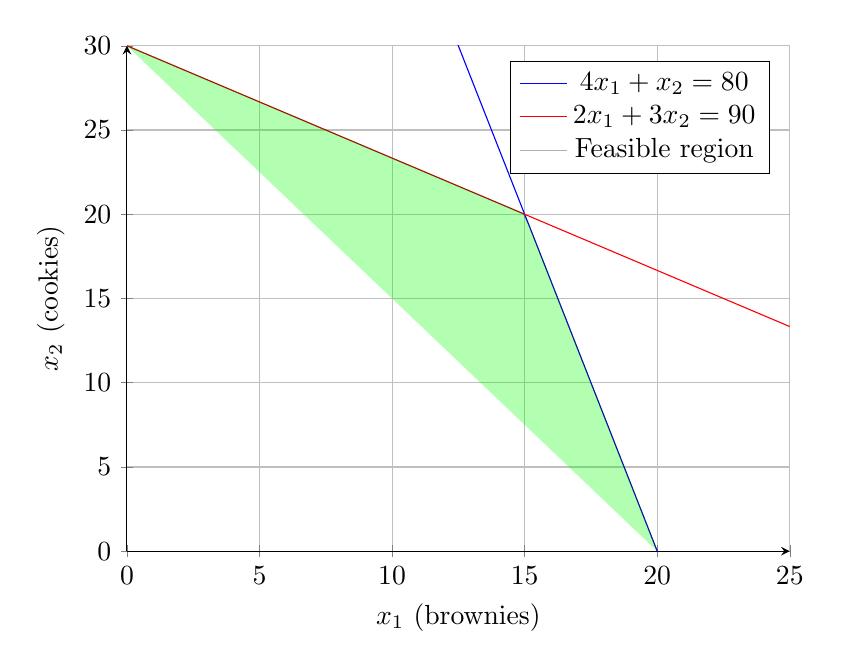
\begin{tikzpicture}
    \begin{axis}[
        axis lines = left,
        xlabel = \(x_1\) (brownies),
        ylabel = \(x_2\) (cookies),
        xmin=0, xmax=25,
        ymin=0, ymax=30,
        grid=major,
        width=10cm,
        height=8cm,
        legend pos=north east
    ]

    % Plotting the constraints
    \addplot [
        domain=0:25, 
        samples=100, 
        color=blue,
    ]
    {80 - 4*x};
    \addlegendentry{\(4x_1 + x_2 = 80\)}

    \addplot [
        domain=0:25, 
        samples=100, 
        color=red,
    ]
    {(90 - 2*x)/3};
    \addlegendentry{\(2x_1 + 3x_2 = 90\)}

    % Highlighting the feasible region
    \addplot [
        domain=0:20, 
        samples=100, 
        fill=green, 
        opacity=0.3,
    ]
    {min(80 - 4*x, (90 - 2*x)/3)};
    \addlegendentry{Feasible region}

    \end{axis}
\end{tikzpicture}
\end{center}

The Simplex method will guide us toward the optimal solution, which lies at one of the vertices of the feasible region.

\subsection*{(b) Range of \( P \) Values for Optimal Solutions}

Now, suppose that the profit per brownie batch is \( P \) dollars, while the profit per cookie batch remains \$30. The new objective function becomes:
\[
\text{Maximize } P x_1 + 30 x_2
\]
We want to determine the range of \( P \) values that make each vertex of the feasible region the optimal solution.

\subsubsection*{Vertices of the Feasible Region}

From part (a), the vertices of the feasible region can be calculated by solving the system of linear equations for each intersection of constraints:
\begin{itemize}
    \item Intersection of \( 4x_1 + x_2 = 80 \) and \( 2x_1 + 3x_2 = 90 \)
    \[
    \text{Solve: } 4x_1 + x_2 = 80 \quad \text{and} \quad 2x_1 + 3x_2 = 90
    \]
    \[
    \text{Solution: } (x_1, x_2) = (15, 20)
    \]
    \item Intersection of \( 4x_1 + x_2 = 80 \) and \( x_2 = 0 \)
    \[
    x_1 = 20, x_2 = 0
    \]
    \item Intersection of \( 2x_1 + 3x_2 = 90 \) and \( x_1 = 0 \)
    \[
    x_1 = 0, x_2 = 30
    \]
    \item Origin: \( (x_1, x_2) = (0, 0) \)
\end{itemize}

\subsubsection*{Range of \( P \) Values for Optimality}

For each vertex, we find the range of \( P \) values where that vertex remains the optimal solution:
\begin{itemize}
    \item At \( (15, 20) \), the objective is \( 15P + 30 \times 20 = 15P + 600 \).
    \item At \( (20, 0) \), the objective is \( 20P \).
    \item At \( (0, 30) \), the objective is \( 30 \times 30 = 900 \).
\end{itemize}

To find the range of \( P \) where each vertex is optimal, we compare these objective values. For example:
\begin{itemize}
    \item \( (20, 0) \) is optimal if \( 20P > 900 \), i.e., \( P > 45 \).
    \item \( (0, 30) \) is optimal if \( 900 > 20P \), i.e., \( P < 45 \).
    \item \( (15, 20) \) is optimal for intermediate \( P \) values where \( 15P + 600 \geq 900 \) and \( 15P + 600 \geq 20P \).
\end{itemize}

Thus, the range of \( P \) values for each vertex is:
\begin{itemize}
    \item Vertex \( (20, 0) \): optimal for \( P > 45 \).
    \item Vertex \( (15, 20) \): optimal for \( 30 \leq P \leq 45 \).
    \item Vertex \( (0, 30) \): optimal for \( P < 30 \).
\end{itemize}


\newpage


\section*{Q6 Simply Simplex}

We are given the following linear program:

\[
\text{Maximize } 5x + 4y
\]
subject to:
\[
\begin{aligned}
    x + 3y &\leq 15 \\
    3x - 2y &\leq 12 \\
    4x + 4y &\geq 16 \\
    x &\geq 0, \quad y \geq 0
\end{aligned}
\]

\subsection*{(a) Sketch the Feasible Region}

We begin by sketching the feasible region. We will first graph the lines corresponding to the constraints and then identify the feasible region.

The constraints are:
\begin{itemize}
    \item \( x + 3y = 15 \), or \( y = \frac{15 - x}{3} \)
    \item \( 3x - 2y = 12 \), or \( y = \frac{3x - 12}{2} \)
    \item \( 4x + 4y = 16 \), or \( y = 4 - x \)
    \item \( x \geq 0 \), \( y \geq 0 \)
\end{itemize}

\begin{center}
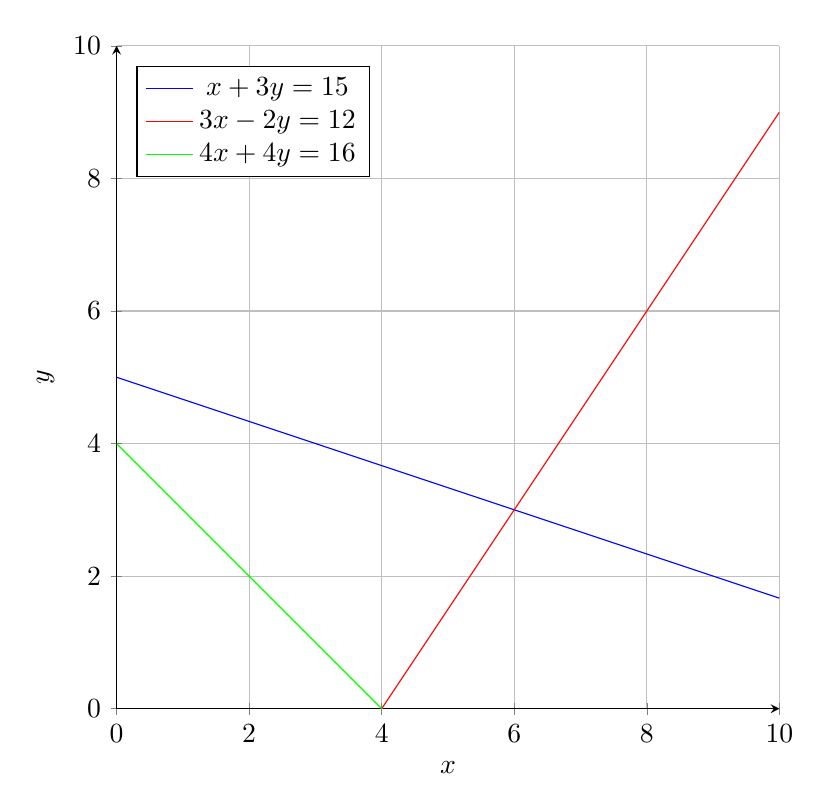
\begin{tikzpicture}
    \begin{axis}[
        axis lines = left,
        xlabel = \(x\),
        ylabel = \(y\),
        xmin=0, xmax=10,
        ymin=0, ymax=10,
        grid=major,
        width=10cm,
        height=10cm,
        legend pos=north west
    ]
    
    % Plotting the constraints
    \addplot [
        domain=0:10, 
        samples=100, 
        color=blue,
    ]
    {(15 - x)/3};
    \addlegendentry{\(x + 3y = 15\)}

    \addplot [
        domain=0:10, 
        samples=100, 
        color=red,
    ]
    {(3*x - 12)/2};
    \addlegendentry{\(3x - 2y = 12\)}

    \addplot [
        domain=0:10, 
        samples=100, 
        color=green,
    ]
    {4 - x};
    \addlegendentry{\(4x + 4y = 16\)}

    \end{axis}
\end{tikzpicture}
\end{center}

The feasible region is the area that satisfies all the constraints and is bounded by the lines we have plotted.

\subsection*{(b) Simplex Algorithm Starting at \( (0,4) \)}

We are asked to run the Simplex algorithm starting at the point \( (0,4) \). First, we need to find the vertices of the feasible region, as the Simplex method moves from vertex to vertex along the edges of the feasible region.

\subsubsection*{Vertices of the Feasible Region}

We calculate the vertices by solving for the intersections of the constraint lines:
\begin{itemize}
    \item Intersection of \( x + 3y = 15 \) and \( 4x + 4y = 16 \):
    \[
    \begin{aligned}
        x + 3y &= 15 \\
        4x + 4y &= 16 \quad \Rightarrow \quad y = 4 - x
    \end{aligned}
    \]
    Substitute \( y = 4 - x \) into \( x + 3y = 15 \):
    \[
    x + 3(4 - x) = 15 \quad \Rightarrow \quad x = 3, y = 1
    \]
    Thus, one vertex is \( (3, 1) \).
    
    \item Intersection of \( 3x - 2y = 12 \) and \( 4x + 4y = 16 \):
    \[
    \begin{aligned}
        3x - 2y &= 12 \\
        4x + 4y &= 16 \quad \Rightarrow \quad y = 4 - x
    \end{aligned}
    \]
    Substitute \( y = 4 - x \) into \( 3x - 2y = 12 \):
    \[
    3x - 2(4 - x) = 12 \quad \Rightarrow \quad x = 4, y = 0
    \]
    Thus, another vertex is \( (4, 0) \).

    \item Intersection of \( x + 3y = 15 \) and \( 3x - 2y = 12 \):
    \[
    \begin{aligned}
        x + 3y &= 15 \\
        3x - 2y &= 12
    \end{aligned}
    \]
    Solve the system of equations:
    \[
    x + 3y = 15 \quad \Rightarrow \quad x = 15 - 3y
    \]
    Substitute into the second equation:
    \[
    3(15 - 3y) - 2y = 12 \quad \Rightarrow \quad y = 3, x = 6
    \]
    Thus, another vertex is \( (6, 3) \).
\end{itemize}

The vertices of the feasible region are \( (3, 1) \), \( (4, 0) \), and \( (6, 3) \).

\subsubsection*{Running the Simplex Algorithm}

Starting at \( (0, 4) \), the objective function is \( 5x + 4y \), so we calculate the objective at each vertex:

\begin{itemize}
    \item At \( (0, 4) \), \( 5(0) + 4(4) = 16 \)
    \item At \( (3, 1) \), \( 5(3) + 4(1) = 15 + 4 = 19 \)
    \item At \( (4, 0) \), \( 5(4) + 4(0) = 20 \)
    \item At \( (6, 3) \), \( 5(6) + 4(3) = 30 + 12 = 42 \)
\end{itemize}

Thus, the maximum value of the objective function is \( 42 \) at \( (6, 3) \), which is the optimal solution.

\end{document}
